%% 
%% Copyright 2007, 2008, 2009 Elsevier Ltd
%% 
%% This file is part of the 'Elsarticle Bundle'.
%% ---------------------------------------------
%% 
%% It may be distributed under the conditions of the LaTeX Project Public
%% License, either version 1.2 of this license or (at your option) any
%% later version.  The latest version of this license is in
%%    http://www.latex-project.org/lppl.txt
%% and version 1.2 or later is part of all distributions of LaTeX
%% version 1999/12/01 or later.
%% 
%% The list of all files belonging to the 'Elsarticle Bundle' is
%% given in the file `manifest.txt'.
%% 

%% Template article for Elsevier's document class `elsarticle'
%% with numbered style bibliographic references
%% SP 2008/03/01

%%\documentclass[preprint,12pt]{elsarticle}

%% Use the option review to obtain double line spacing
%% \documentclass[authoryear,preprint,review,12pt]{elsarticle}

%% Use the options 1p,twocolumn; 3p; 3p,twocolumn; 5p; or 5p,twocolumn
%% for a journal layout:
%% \documentclass[final,1p,times]{elsarticle}
%% \documentclass[final,1p,times,twocolumn]{elsarticle}
%% \documentclass[final,3p,times]{elsarticle}
%% \documentclass[final,3p,times,twocolumn]{elsarticle}
%% \documentclass[final,5p,times]{elsarticle}
\documentclass[final,5p,times,twocolumn]{elsarticle}

%% For including figures, graphicx.sty has been loaded in
%% elsarticle.cls. If you prefer to use the old commands
%% please give \usepackage{epsfig}

%% The amssymb package provides various useful mathematical symbols
%\usepackage{amssymb}
%% The amsthm package provides extended theorem environments
%% \usepackage{amsthm}

%% The lineno packages adds line numbers. Start line numbering with
%% \begin{linenumbers}, end it with \end{linenumbers}. Or switch it on
%% for the whole article with \linenumbers.
%% \usepackage{lineno}
%% \modulolinenumbers[5]


\usepackage{hyperref}


%\journal{Nuclear Physics B}
%%%%%%%%%%%%%%%%%%%%%%%
%% To change the style, put a % in front of the second line of the current style and
%% remove the % from the second line of the style you would like to use.
%%%%%%%%%%%%%%%%%%%%%%%

%% Numbered
%\bibliographystyle{model1-num-names}

%% Numbered without titles
%\bibliographystyle{model1a-num-names}

%% Harvard
%\bibliographystyle{model2-names.bst}\biboptions{authoryear}

%% Vancouver numbered
%\usepackage{numcompress}\bibliographystyle{model3-num-names}

%% Vancouver name/year
%\usepackage{numcompress}\bibliographystyle{model4-names}\biboptions{authoryear}

%% APA style
%\bibliographystyle{model5-names}\biboptions{authoryear}

%% AMA style
%\usepackage{numcompress}\bibliographystyle{model6-num-names}

%% `Elsevier LaTeX' style
\bibliographystyle{elsarticle-num}
%%%%%%%%%%%%%%%%%%%%%%%

%%%%%%%%%%%%%%%%%%%%%%%%%%%%%%%%%%  Format source code
\usepackage{color}
\usepackage{graphicx,grffile}
\setlength{\emergencystretch}{3em}  % prevent overfull lines
\usepackage{fancyvrb}
\newcommand{\VerbBar}{|}
\newcommand{\VERB}{\Verb[commandchars=\\\{\}]}
\DefineVerbatimEnvironment{Highlighting}{Verbatim}{commandchars=\\\{\}}
% Add ',fontsize=\small' for more characters per line
\newenvironment{Shaded}{}{}
\newcommand{\KeywordTok}[1]{\textcolor[rgb]{0.00,0.44,0.13}{\textbf{{#1}}}}
\newcommand{\DataTypeTok}[1]{\textcolor[rgb]{0.56,0.13,0.00}{{#1}}}
\newcommand{\DecValTok}[1]{\textcolor[rgb]{0.25,0.63,0.44}{{#1}}}
\newcommand{\BaseNTok}[1]{\textcolor[rgb]{0.25,0.63,0.44}{{#1}}}
\newcommand{\FloatTok}[1]{\textcolor[rgb]{0.25,0.63,0.44}{{#1}}}
\newcommand{\ConstantTok}[1]{\textcolor[rgb]{0.53,0.00,0.00}{{#1}}}
\newcommand{\CharTok}[1]{\textcolor[rgb]{0.25,0.44,0.63}{{#1}}}
\newcommand{\SpecialCharTok}[1]{\textcolor[rgb]{0.25,0.44,0.63}{{#1}}}
\newcommand{\StringTok}[1]{\textcolor[rgb]{0.25,0.44,0.63}{{#1}}}
\newcommand{\VerbatimStringTok}[1]{\textcolor[rgb]{0.25,0.44,0.63}{{#1}}}
\newcommand{\SpecialStringTok}[1]{\textcolor[rgb]{0.73,0.40,0.53}{{#1}}}
\newcommand{\ImportTok}[1]{{#1}}
\newcommand{\CommentTok}[1]{\textcolor[rgb]{0.38,0.63,0.69}{\textit{{#1}}}}
\newcommand{\DocumentationTok}[1]{\textcolor[rgb]{0.73,0.13,0.13}{\textit{{#1}}}}
\newcommand{\AnnotationTok}[1]{\textcolor[rgb]{0.38,0.63,0.69}{\textbf{\textit{{#1}}}}}
\newcommand{\CommentVarTok}[1]{\textcolor[rgb]{0.38,0.63,0.69}{\textbf{\textit{{#1}}}}}
\newcommand{\OtherTok}[1]{\textcolor[rgb]{0.00,0.44,0.13}{{#1}}}
\newcommand{\FunctionTok}[1]{\textcolor[rgb]{0.02,0.16,0.49}{{#1}}}
\newcommand{\VariableTok}[1]{\textcolor[rgb]{0.10,0.09,0.49}{{#1}}}
\newcommand{\ControlFlowTok}[1]{\textcolor[rgb]{0.00,0.44,0.13}{\textbf{{#1}}}}
\newcommand{\OperatorTok}[1]{\textcolor[rgb]{0.40,0.40,0.40}{{#1}}}
\newcommand{\BuiltInTok}[1]{{#1}}
\newcommand{\ExtensionTok}[1]{{#1}}
\newcommand{\PreprocessorTok}[1]{\textcolor[rgb]{0.74,0.48,0.00}{{#1}}}
\newcommand{\AttributeTok}[1]{\textcolor[rgb]{0.49,0.56,0.16}{{#1}}}
\newcommand{\RegionMarkerTok}[1]{{#1}}
\newcommand{\InformationTok}[1]{\textcolor[rgb]{0.38,0.63,0.69}{\textbf{\textit{{#1}}}}}
\newcommand{\WarningTok}[1]{\textcolor[rgb]{0.38,0.63,0.69}{\textbf{\textit{{#1}}}}}
\newcommand{\AlertTok}[1]{\textcolor[rgb]{1.00,0.00,0.00}{\textbf{{#1}}}}
\newcommand{\ErrorTok}[1]{\textcolor[rgb]{1.00,0.00,0.00}{\textbf{{#1}}}}
\newcommand{\NormalTok}[1]{{#1}}
%%%%%%%%%%%%%%%%%%%%%%%%%%%%%%%%%%  Format source code

\begin{document}

\begin{frontmatter}

\title{Forensic-Tool Development with Rust}

%\title{Forensic-Tool Development with Rust\tnoteref{mytitlenote}}
%\tnotetext[mytitlenote]{Fully documented templates are available in the elsarticle package on \href{http://www.ctan.org/tex-archive/macros/latex/contrib/elsarticle}{CTAN}.}

%% Group authors per affiliation:
%\author{Elsevier\fnref{myfootnote}}
%\address{Radarweg 29, Amsterdam}
%\fntext[myfootnote]{Since 1880.}

%% or include affiliations in footnotes:
%\author[mymainaddress,mysecondaryaddress]{Elsevier Inc}
%\ead[url]{www.elsevier.com}

%\author[mysecondaryaddress]{Global Customer Service\corref{mycorrespondingauthor}}
%\cortext[mycorrespondingauthor]{Corresponding author}
%\ead{support@elsevier.com}

%\address[mymainaddress]{1600 John F Kennedy Boulevard, Philadelphia}
%\address[mysecondaryaddress]{360 Park Avenue South, New York}

\author{Jens Getreu}
\author{Olaf Maennel}
\address{Tallinn University of Technology, Ehitajate tee 5, 19086 Tallinn,
Estonia} 

\begin{abstract}
The study evaluates the suitability of the \emph{Rust} ecosystem
for forensic tool development.  As a case study a forensic tool
named \emph{Strings­ext}\cite{getreu2017a}\cite{getreu2017} is developed. 
Starting from analysing the specific requirements of forensic software
in general and those of the present case study, all stages of the software
development life-cycle are executed and evaluated.
\emph{Strings­ext} is a reimplementation and enhancement of the
\emph{GNU-strings} tool, a widely used program in forensic investigations.
\emph{Strings­ext} recognizes Cyrillic, CJKV East Asian characters and other
scripts in all supported multi-byte-encodings while \emph{GNU-strings} fails in
finding these in UTF-16 and other encodings.

During the case study it has become apparent that the \emph{Rust}
ecosystem provides good support for secure coding principles and unit
testing. Furthermore, the benchmarks showed a satisfactory performance
of the resulting \emph{Strings­ext} binaries comparable to the original
\emph{C} version.
\end{abstract}


\begin{keyword}

Forensic analysis, string search, multibyte encoding, Rust
language, \texttt{Stringsext}-tool

\end{keyword}

\end{frontmatter}

%\linenumbers


%%%%%%%%%%%%%%%%%%%%%%%%%%%%%%%%%%%%%%%%%%%%%%%%%%%%%%%%%%%%%%%%%%%%%%%%%%5






\section{Introduction}

Human interaction with electronic devices leaves traces in their electronic
memory. In the age of cloud computing most human interaction triggers requests
to distant servers leaving traces not only in their log files, but also in many
intermediate network devices. Due to the cross-linked nature of computer systems
the data that needs to be taken into consideration when investigating a crime is
enormous. In this huge amount of information the investigator has to find those
specific bits of information constituting digital evidences. 

In the domain of digital forensics an electronic trace (observation) with a
well-known cause-effect-relationship between the observation and the human
action causing it (activity), is a so called \textbf{artefact}.  \footnote{For
the sake of simplicity we present here a rather simplistic view associating
univocally one trace (artefact/observation) with only one possible
cause/activity. In the physical world, one trace might have several possible
causes which cannot be excluded a priori. For this reason modern forensics
favours the \emph{Likelihood Ratio} approach, in which the degree of support of
the observations for the hypotheses is considered, providing a strength of
evidence (diagnostic value) that is relative to the hypotheses tested.} It
embodies any ``item of interest that helps an investigation move forward.''
\cite[p. 125]{harichandran2016}\footnote{Cf. Harichandran \cite[p.
131]{harichandran2016} who proposed a more formal definition: A \emph{Curated
(digital) Forensic Artefact (CuFA)} ''must have evidentiary value in a legal
proceeding, must be created by an external force/artificially, must have
antecedent temporal relation/importance and must be exceptional (based on
accident, rarity, or personal interest)[...]``.}.

Forensic examiners - the law enforcement personnel who deal with 
digital evidence - face inter alia two challenges: to collect and to 
preserve the huge amount of data that may be related to a crime and to 
search and detect artefacts in the collected data.

The latter aspect implies the so called \emph{string search} which is useful
when dealing with unknown binary data. Most binary data contain human readable
character sequences called strings. A very commonly used program to extract
strings from a binary data is the so called \emph{GNU-strings} program. The
software tool \emph{Stringsext}, developed in this present work, is made for
same purpose. The new development is designed to overcome some of
\emph{GNU-strings} shortcomings. Where possible, it maintains
\emph{GNU-strings'} user-interface.

In the following section we analyse general tool requirements in digital 
forensics. Together with the shortcomings of the original  
\emph{GNU-strings} tool, it become obvious that the C++ programming language
does not satisfy the indispensable security requirements in the field of
forensic software. The section \emph{}



\section{Tool Requirements in Digital Forensics}
\label{sec:tool-requirements}

\subsection{Multi-byte character encoding support}
\label{subsec:tool-validation}

Like in other established forensic disciplines the forensic soundness and
reliability of digital evidence depend on the validity and correctness of the
forensic software used in examination. In other words, to guarantee that the
digital evidence is forensically sound, all tools used to collect, preserve and
analyse digital evidences must be validated. Tool validation can also be
formally required to comply with standards like the \emph{ISO 17025 Laboratory
Accreditation standard}.


\begin{description}
\item[Validation]
    is the confirmation by examination and the provision of objective
    evidence that a tool, technique or procedure functions correctly and as
    intended.\cite[p. 92]{craiger2006}.
\end{description}


One way of establishing a set of requirements for a new forensic tool is to
analyse how similar existing tools are validated. Beckett and Slay
\cite{beckett2007} propose a \emph{functionality oriented validation} method
called \emph{Model of tool neutral testing}. Instead of testing if a software
product meets all its requirements, an independent set of forensic functions is
defined and later tested. The digital forensic discipline can be broadly defined
in terms of the key functions \emph{Identification, Data Preservation, Data
Analysis and Presentation of Digital Evidence}. Each key function is further
divided into subcategories. For example \emph{Data Analysis} breaks down into:
\emph{Searching, File Rendering, Data Recovery, Decryption, Identification,
Processing, Temporal Data} and \emph{Process Automation}.  The first item
\emph{searching} relates to finding and locating the information of interest in
digital memories. Form a functional point of view the \emph{searching} falls
into the searching domain (where), the searching mode (how) and the searching
target (what). The breakdown of forensic functions into detailed categories
allows to decouple the validation procedure from the implementation of the
forensic tool itself. Based on this categorisation, independent test
environments are set up for each specific function. For example a
test may certify if the software is able to run a fuzzy search for strings in
the unallocated disk space.

Beyond validation, the categorisation of forensic functions is also helpful to
analyse existing tools - in our case \emph{GNU strings} - in oder to define
requirements for improvement.  For example, \emph{Searching} can be further
classified into groups as shown in the Figure \ref{the-search-target-mapping}
\cite[p. 17]{beckett2007}. The leaves in the diagram list capabilities a
\emph{Searching}-software can implement.  For example the subcategory
``Character encoding'' illustrates the main deficit of \emph{GNU-strings} as it
supports only ASCII encoding. In a global cyberspace, forensic tools must
identify a multitude of encodings. This leads us to the main motivation and
requirement of \emph{Strings­ext}: \emph{multibyte character encoding support}.

\begin{figure}[htbp]
\centering
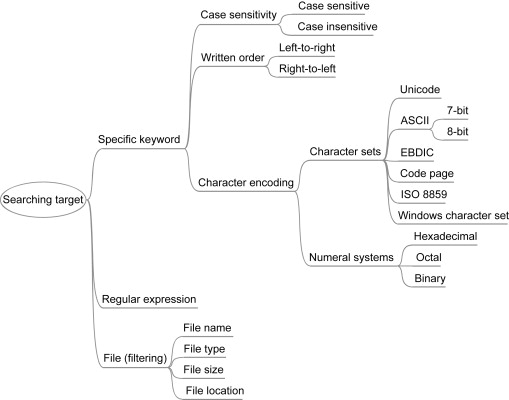
\includegraphics[width=\linewidth]{images/03-The_search_target_mapping.jpg}
	\caption{The search target mapping \protect\cite[p. 17]{beckett2007}}
	\label{the-search-target-mapping}
\end{figure}

The \emph{functionality oriented validation} can be classified as ``black box
testing'' examining functionality without any knowledge of the internal
implementation, even without having access to the source code. One advantage is,
that it allows to reuse the test environment thus reducing costs. Black box
testing is sometimes also referred as ``behavioural testing'' as it feeds the
tool with a known test case data and observes if the tool outputs the expected
results. In the context of this work black box testing is used to assert that
the developed tool \emph{Stringsext} deals correctly with big real-world input
data: \emph{Stringsext} has been designed to produce, as a special case,
bit-identical output to that of \emph{GNU-strings}.  This way the comparison of
the output data of both tools allowed to confirm that \emph{stringsext} is
working correctly when dealing with big data. 

In addition to the above black box testing, Rust's build in test harness (unit
test) is used in conjunction with the \emph{test driven development} in order
to guarantee maximum security and correctness of the developed tool.



\subsection{Security}
\label{subsec:security1}


``Make it hard for them to find you and impossible for them to prove they found
you''. With this concise word Berinato\cite{berinato2007} characterises the
relation between the criminal and the forensic investigator. In digital
forensics this "hide-and-seek" game might soon take a new dimension: Eggendorfer
\cite{eggendorfer2016} stresses with good reasons that forensic tools are
software too and therefor vulnerable to attacks: A vulnerability found in 2017
in a common forensic tool \emph{EnCase Forensic Imager} demonstrates exemplary
the pertinence of the risk \cite{secconsult2017}: 

\begin{quote}
    \emph{By writing a manipulated LVM2 partition (a hard disk format commonly
    used for Linux servers) on a storage device, an attacker could - if the
    device were ever to be analysed using EnCase Forensic Imager - take over an
    investigator's machine. When the investigator tries to read the device,
    EnCase Forensic Imager crashes - unbeknownst to the investigator, however, a
    lot more is happening. Through a buffer overflow security flaw, EnCase
    Forensic Imager can be tricked into executing data read from the storage
    device. Afterwards the code provided by the attacker has full control of the
    investigator's machine and can be used by the suspect to manipulate evidence
    \cite{secconsult2017}.}
\end{quote}

Confronted with this vulnerability report, the vendor downgraded the issue: "The
exploit SEC Consult claims to have found is an extreme edge case, much like the
theoretical alerts they tried to promote in November. [...] We do not consider
this claim to be serious and it will not impact the performance of our products
\cite{secconsult2017}." For the user it remains unclear if and when the
vulnerability gets fixed. While such a reaction would have been inconceivable in
other software domains, the risk of forensic tool exploitation is still largely
neglected despite its potential impact:

\begin{itemize} 

    \item The adversary can be warned about an ongoing investigation.

    \item The adversary can gain control of the investigator's machine
        and alter evidences.

\end{itemize}

The\emph{Stringsext}-project addresses this risk by choosing the programming
language Rust. Rust offers some outstanding security guarantees which are
presented in Section \ref{rust-lang}.


\subsection{Code efficiency}
\label{subsec:code-efficiency}

The searching domain in forensic investigations is often as large as the seized
data-carrier. Nowadays hard-disk images hold several TiB of data.  Memory images
of the RAM are smaller, but still some GiB in size. In order to address so big
search domains, forensic software must operate very efficiently. This is why
forensic software is often programmed in C or C++. But not only the programming
language matters: Efficient code requires carefully chosen abstractions,
efficient algorithms avoiding unnecessary data-copies and program-loops.
Concerning the choice of the programming language we define the following
requirements. The programming language 

\begin{itemize}
\item
  allows a fine control over pointers and memory allocation,
\item
  offers zero cost abstractions,
\item
  has no or minimal runtime.
\end{itemize}


\noindent
The above motivates the choice of developing \emph{Stringsext} in Rust.
Chapter \ref{rust-lang} shows how Rust meets the above requirements by its
\emph{memory safety} guarantees and \emph{zero cost} design goal. 


\section{\emph{GNU-strings}' shortcomings in forensics}
\label{sec:strings-and-forensics}

This chapter first analyses \emph{GNU-strings'} limitations concerning
multi-byte-encodings and international scripts. Based
upon this we derive a set of additional requirements for \emph{Strings­ext}.

Many forensic practitioners  use the GNU program \emph{strings}, hereafter
referred as \emph{GNU strings}, to get a sense of the functionality of an
unknown program by extracting human readable strings from binary data. Of
special interest are for example strings containing URLs to malicious sites,
often an indicator of malware activity. Also, user prompts, error
messages, and status messages can give valuable hints.


\subsection{Test case - International character encodings}
\label{subsec:test-case-strings}

As discussed above the main motivation for developing \emph{Strings­ext} is the
missing multi-byte character encoding semantics in \emph{GNU-strings}.
\emph{GNU-strings} encoding support consists of a rudimentary filter accessed
with the option \texttt{-\/-encoding}. Please consult the manual page for more
details. How well does \emph{GNU-strings} detect Unicode?  The Figure
\ref{fig:test-international-character-encodings} shows the content of a text
file chosen as test case.

\begin{figure}[htbp]
   \centering
   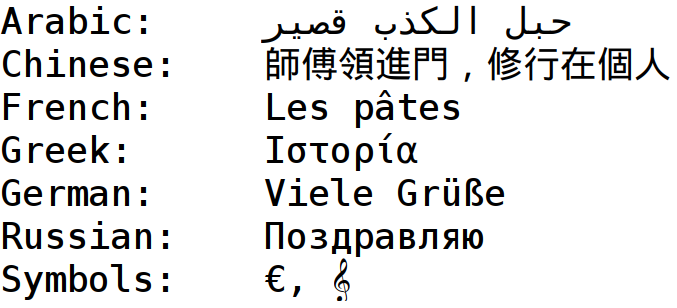
\includegraphics[width=0.6\linewidth]{images/test_case_encoding-input.png}
   \caption{Test case international character encodings}
   \label{fig:test-international-character-encodings}
\end{figure}

To find out how well \emph{GNU Strings} deals with different encodings, the
text-file is then is converted into \texttt{UTF-8}, \texttt{UTF-16LE},
\texttt{UTF-16BE}, \texttt{UTF-32LE} and \texttt{UTF-32BE}, each encoding in one
file.  In order to observe \emph{GNU-strings} Unicode detection capabilities,
all the test-files are then searched for valid graphic strings with the command
\texttt{strings} using all possible variation of its encoding filter.  The
Figure \ref{fig:strings-e-l} shows exemplary \emph{GNU-strings} output for an
UTF-16 little endian encoded input.
 

\begin{figure}[htbp]
\centering

\includegraphics[width=0.7\linewidth]{images/strings_-e_l.png}
\caption{GNU-strings with UTF-16LE encoded input}
\label{fig:strings-e-l}
\end{figure}


\noindent \textbf{Results:} \texttt{UTF-8} is the only encoding in which
\emph{GNU strings} is able to find international characters.  The Figure
\ref{fig:strings-e-l}, chosen as an example, shows that with \texttt{UTF-16}
input, \emph{GNU strings} fails to recognize all non-ASCII characters.  The same
holds true for \texttt{UTF-32} and most other encodings: This limitation is of
particular importance in forensic investigations: The Microsoft-Windows
operating system handles Unicode characters in memory as 2 byte \texttt{UTF-16}
words. As a result when dealing with Microsoft-Windows memory images,
\emph{GNU-strings} is not able to detect any international characters!  It
should not be forgotten that \emph{GNU-strings} is not designed to analyse
multi-byte encodings in general.  This is why other very common encodings e.g.
\emph{big5} or \emph{koi8-r} are not supported at all even though they are
widely used.  The above-outlined limitations leads to \emph{Strings­ext}'s main
requirement: \emph{character encoding support}.



\subsection{Secure coding}\label{security2}

In the narrow sense, ``secure coding'' is rather a design goal than a functional
requirement. Secure coding denotes the practice of developing computer software
by reducing the accidental introduction of security vulnerabilities 
by preventing coding errors or discovering and eliminating
security flaws during implementation and testing.  From the code security point
of view the requirement \emph{character encoding support} is the most critical:
The NIST \emph{National Vulnerability Database} lists under the heading
``character encoding'' 22 vulnerabilities.  Not only new complex forensic
software is affected by vulnerabilities. It also concerns other well-established
products: The tool \emph{GNU-strings}, part of the \emph{GNU binutils}
collection, became publicly available in 1999 \cite{cygnussolutions1999}.
Today it has reached the notable age of 17 years. \emph{GNU-strings} is a
comparatively small program with 724 lines of code only. It is all the more
surprising that in 2014 the security researcher Zalewski discovered a serious
security vulnerability \emph{CVE-2014-8485} \cite{zalewski2014}:

\begin{quote}
   \emph{The setup\_group function in \texttt{bfd/elf.c} in \texttt{libbfd} in
   GNU binutils 2.24 and earlier allows remote attackers to cause a denial of
   service (crash) and possibly execute arbitrary code via crafted section
   group headers in an ELF file.}
\end{quote}

Zalewski headlined his bug report ``Don't run strings on untrusted
files.'' Needless to say that this advice can not be followed in the
context of a forensic investigation. In the meantime the bug was fixed
but users remain confused and bewildered.

Of particular importance is that the above bugs are part of a vulnerability
class related to memory safety problems. \emph{GNU strings} is written in C, a
language whose abstractions can not guarantee memory safety. In order to exclude
potential vulnerabilities of the same kind from the start, \emph{Strings­ext}
was developed in the \emph{Rust} programming language.



\section{The Rust programming language}\label{rust}
\label{rust-lang}

In the Section \ref{sec:tool-requirements} we showed that the requirements
\emph{code efficiency} and \emph{security} are of paramount importance. 
This section illustrates how Rust supports these requirements with
its \emph{zero cost abstractions} and its \emph{guaranteed memory safety}
motivating the choice of implementing \emph{Strings­ext} in Rust.

\subsection{Memory safety}\label{_memory_safety}

All memory-related problems in \emph{C} and \emph{C++} come from the
fact that \emph{C} programs can unrestrainedly manipulate pointer to
variables and objects outside of their memory location and their
lifetime. The Table \ref{tab:c-memory-safety-bugs}
shows a selection of most common memory safety related vulnerabilities
\cite{mitrecorporation2016}. Memory
safe languages like \emph{Java} do not give programmers direct and
uncontrolled access to pointers. For example, in \emph{Java} 
memory safety is guaranteed through 
a resource costly runtime and a garbage collector. The related
additional costs in terms of runtime resources exclude programming
language like Java for most forensic tool development.

\begin{table}[htbp]
\begin{center}
\begin{tabular}{ | l  p{6.5cm} | }
\hline
CWE	& ID Name \\ \hline
\hline
119	& Improper Restriction of Operations within the Bounds of a Memory 
      Buffer\\ \hline
120 & Buffer Copy without Checking Size of Input ('Classic Buffer 
      Overflow')\\ \hline
125 & Out-of-bounds Read\\ \hline
126 & Buffer Over-read ('Heartbleed bug')\\ \hline
122 & Heap-based Buffer Overflow\\ \hline
129 & Improper Validation of Array Index\\ \hline
401 & Improper Release of Memory Before Removing Last Reference ('Memory 
      Leak')\\ \hline
415 & Double Free\\ \hline
416 & Use After Free\\ \hline
591 & Sensitive Data Storage in Improperly Locked Memory\\ \hline
763 & Release of Invalid Pointer or Reference\\ \hline
\end{tabular}
\end{center}
    \caption{Common weaknesses in C/C++ that affect memory}
    \label{tab:c-memory-safety-bugs}
\end{table}


For many years program efficiency and memory safety seemed to be an
insurmountable discrepancy. Now, after 10 years of development, a new
programming language called \emph{Rust} promises to cope with this balancing
act. \emph{Rust}'s main innovation is the introduction of semantics defining
\emph{data ownership}. This new programming paradigm allows the compiler to
guarantee memory safety at \emph{compile-time}.  Thus, no resource costly
runtime is needed for that purpose. In \emph{Rust} most of the weaknesses listed
in Table \ref{tab:c-memory-safety-bugs} are already detected at compile time.
Moreover, the \emph{Rust} compiler guarantees that none of these weaknesses
can result in an undefined system state or provoke data leakage.

\emph{Rust}'s main innovation is the introduction of new semantics defining
\emph{ownership} and \emph{borrowing}. Put in simplified terms, they
translate to the following three rules which Rust's type system enforces at
compile time:

\begin{enumerate}
\def\labelenumi{\arabic{enumi}.}
\item
  All resources (everything that can be bound to a variable, e.g.
  vectors etc.) have a sole owner.

\item Others can borrow from the owner (technically borrowing means that another
scope sets a pointer to the owner's ressource). 

\item
  The owner cannot free or mutate the resource while it is borrowed.
\end{enumerate}

By enforcing the above rules \emph{Rust} organizes how resources are shared
among different scopes. Memory problems occur for instance when a resource is
referenced by multiple pointers (aliasing) and when it is mutable at the same
time. In contrast to other languages, \emph{Rust}'s semantics allow the type
system to ensure \emph{at compile time} that simultaneous aliasing and mutation
mutually exclude each other (cf. Table \ref{tab:resource-sharing-in-rust}). As
the check is performed at compile-time, no run-time code is necessary.
Furthermore, \emph{Rust} does not need a garbage collector: when owned data goes
out of scope it is immediately destroyed.

\begin{table}[htbp]
\begin{center}
\begin{tabular}{ | l | l | l | l | }
\hline
    Resource sharing      & Aliasing & Mutation & Example \\
\hline
    move ownership        & no       & yes      & \texttt{let a=b} \\
    shared borrow         & yes      & no       & \texttt{let a=\&b} \\
    mutable borrow        & no       & yes      & \texttt{let a=\&mut b} \\
\hline
\end{tabular}
\end{center}
    \caption{Resource sharing in Rust}
    \label{tab:resource-sharing-in-rust}
\end{table}

The following code samples \cite[Sec. 3.2]{the-rust-project-developers2017}
illustrate how the Rust compiler detects non-obvious hidden memory safety
issues. The function \texttt{as\_str} returns a pointer to a stack allocated
resource \texttt{s} that is freed at the end of the function: we find ourselves
with a ``Use after free'' condition! The compiler aborts with the error message
\texttt{s\ does\ not\ live long\ enough}.
i
\begin{Shaded}
\begin{Highlighting}[]
\KeywordTok{fn} \NormalTok{as_str(data: &}\DataTypeTok{u32}\NormalTok{) -> &}\DataTypeTok{str} \NormalTok{\{}
      \KeywordTok{let} \NormalTok{s = }\PreprocessorTok{format!}\NormalTok{(}\StringTok{"\{\}"}\NormalTok{, data);}
      \NormalTok{&s}
\NormalTok{\}}
\end{Highlighting}
\end{Shaded}

\noindent
Here the corrected memory safe code:


\begin{Shaded}
\begin{Highlighting}[]
\KeywordTok{fn} \NormalTok{as_str(data: &}\DataTypeTok{u32}\NormalTok{) -> }\DataTypeTok{String} \NormalTok{\{}
      \KeywordTok{let} \NormalTok{s = }\PreprocessorTok{format!}\NormalTok{(}\StringTok{"\{\}"}\NormalTok{, data);}
      \NormalTok{s}
\NormalTok{\}}
\end{Highlighting}
\end{Shaded}

\noindent
The \texttt{push()} method in line 3 of the next example causes the backing
storage of \texttt{data} to be reallocated. As a result we have a
dangling pointer vulnerability! Again, the Rust compiler detects the error 
and code does not compile.


\begin{Shaded}
\begin{Highlighting}[]
\KeywordTok{let} \KeywordTok{mut} \NormalTok{data = }\PreprocessorTok{vec!}\NormalTok{[}\DecValTok{1}\NormalTok{, }\DecValTok{2}\NormalTok{, }\DecValTok{3}\NormalTok{];}
\KeywordTok{let} \NormalTok{x = &data[}\DecValTok{0}\NormalTok{];}
\NormalTok{data.push(}\DecValTok{4}\NormalTok{);}
\PreprocessorTok{println!}\NormalTok{(}\StringTok{"\{\}"}\NormalTok{, x);}
\end{Highlighting}
\end{Shaded}

\noindent
Here the corrected memory safe version that compiles:

\begin{Shaded}
\begin{Highlighting}[]
\KeywordTok{let} \KeywordTok{mut} \NormalTok{data = }\PreprocessorTok{vec!}\NormalTok{[}\DecValTok{1}\NormalTok{, }\DecValTok{2}\NormalTok{, }\DecValTok{3}\NormalTok{];}
\NormalTok{data.push(}\DecValTok{4}\NormalTok{);}
\KeywordTok{let} \NormalTok{x = &data[}\DecValTok{0}\NormalTok{];}
\PreprocessorTok{println!}\NormalTok{(}\StringTok{"\{\}"}\NormalTok{, x);}
\end{Highlighting}
\end{Shaded}


\subsection{Iterators}\label{_iterators}

A very common group of programming mistakes is related to improper handling of
indexes especially in loops, e.g. ``CWE-129: Improper Validation of Array
Index'' (cf. Table
\ref{tab:c-memory-safety-bugs2}\cite{mitrecorporation2016}).

\begin{table}[htbp]
\begin{center}
\begin{tabular}{ | l  p{6.5cm} | }
\hline
CWE ID & Name \\
\hline
\hline
119 & Improper Restriction of Operations within the Bounds of a Memory Buffer \\
125 & Out-of-bounds Read \\
129 & Improper Validation of Array Index \\
\hline
\end{tabular}
\end{center}
    \caption{Common weaknesses in C/C++ affecting memory avoidable with 
	     iterators\protect\cite{mitrecorporation2016}}
    \label{tab:c-memory-safety-bugs2}
\end{table}


In addition to traditional imperative loop control structures, \emph{Rust}
offers efficient iteration with functional style iterators.  Like in Haskell
iterators are lazy and avoid allocating memory for intermediate structures (you
allocate just when you call \texttt{.collect()}). Iterators considerably enhance
the robustness and safety of programs. They enable the programmer to iterate
through vectors without explicitly naming neither the index nor its bounds, thus
avoiding related common mistakes. The Figure \ref{fig:cipher} shows an example.


\begin{figure}[htbp]
\begin{Shaded}
\begin{Highlighting}[]
\NormalTok{fet p: }\DataTypeTok{Vec}\NormalTok{<}\DataTypeTok{u8}\NormalTok{> = s.into_bytes(); }\CommentTok{//plaintext}
\KeywordTok{let} \KeywordTok{mut} \NormalTok{c: }\DataTypeTok{Vec}\NormalTok{<}\DataTypeTok{u8}\NormalTok{> = }\PreprocessorTok{vec!}\NormalTok{[];     }\CommentTok{//ciphertext}

\KeywordTok{for} \NormalTok{(cypherb, keyb) }\KeywordTok{in} \NormalTok{p.iter()}
    \NormalTok{.zip(  key.iter().cycle().take(p.len())  ) \{}
        \NormalTok{c.push(*cypherb ^ *keyb }\KeywordTok{as} \DataTypeTok{u8}\NormalTok{);}
    \NormalTok{\}}
\end{Highlighting}
\end{Shaded}
\caption{Vigenère cipher in Rust}
\label{fig:cipher}
\end{figure}

It must be noted that even with iterators \emph{out of bounds}-errors may occur.
Nevertheless, iterators should be preferred because they reduce the probability
of errors related to indexes drastically.


\subsection{Zero-Cost Abstractions}
\label{subsec:zero-cost-abstractions}

It is the language design goal \emph{Zero-Cost Abstractions} that makes the
\emph{C/C++} language so efficient and suitable for system programming. It means
that libraries implementing abstractions, e.g. vectors and strings, must be
designed in a way that the compiled binary is as efficient as if the program had
been written in Assembly. This is best illustrated with memory layouts: Figure
\ref{fig:rust-vec} shows a vector in \emph{Rust}. Its memory layout is very
similar is to a vector in \emph{C/C++}.

\begin{figure}[htbp]
\centering
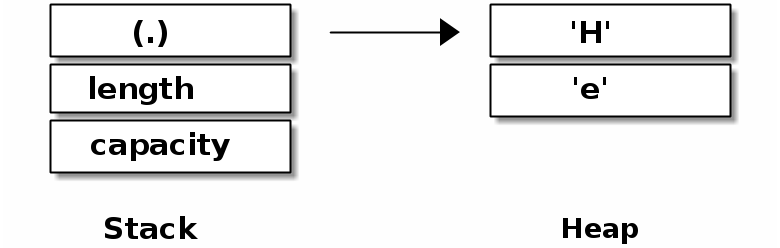
\includegraphics[width=0.6\linewidth]{images/rust-vec.png}
\caption{Memory layout of a Rust vector}
\label{fig:rust-vec}
\end{figure}

In contrast, the memory safe language \emph{Java} enforces a uniform internal
representation of data. In Java a vector has 2 indirections instead of 1
compared to \emph{Rust} and \emph{C/C++} (cf. Fig.  \ref{fig:java-vec}). As the
data could be represented in a more efficient way in memory, we see that
\emph{Java} does not prioritise \emph{Zero-Cost-Abstraction} as primary
objective.

\begin{figure}[htbp]
\centering
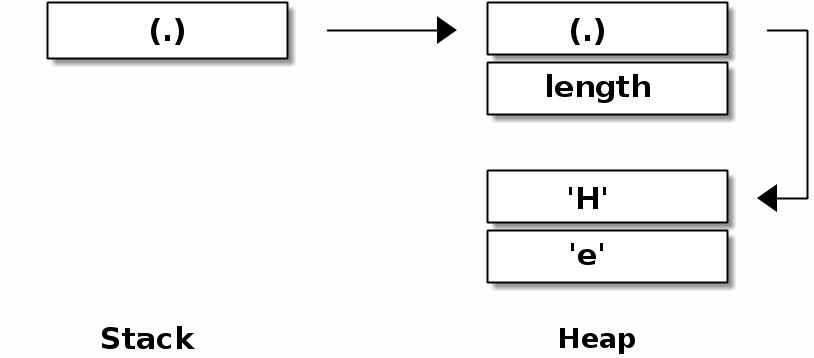
\includegraphics[width=0.6\linewidth]{images/java-vec.png}
\caption{Memory layout of a Java vector}
    \label{fig:java-vec}
\end{figure}


\section{Use case: development of the \emph{Stringsext}-tool}

In the Section \ref{sec:tool-requirements} we have analysed the special
requirements for tools in digital forensics: \emph{code
efficiency} and \emph{security}. The Section \ref{rust-lang}
showed that Rust's core properties \emph{zero cost abstractions} and 
\emph{memory safety} in theory meet well our requirements.

But how well is the Rust ecosystem suited for forensic tool development? In
order to evaluate the practical aspects of Rust we developed the tool
\emph{Stringsext} \cite{getreu2017a}\cite{getreu2017}. The technical challenges
such as concurrent batch processing of multi-byte character streams revealed to
be sufficiently complex, thus allowing us to deduce general recommendations for
forensic-tool development.




\subsection{Concurrency}\label{_concurrency}

The Figure \ref{fig:data-processing-and-threads} shows the data flow in
\emph{Strings­ext}. All \emph{scanner} instances as well as the
\emph{merger-printer} are designed as threads. Rust uses OS-level threads and
its type and ownership model guarantees the absence of data races.  Rust
supports by default two models of inter-thread communication: shared memory
\footnote{Rust inherits C11's memory model for atomics} and message channels.


\emph{Stringsext} imports the crate \texttt{scoped\_threadpool} used to
distribute the \emph{shared-memory} \texttt{input\_slice} to its
scanner-threads. Once a scanner has accomplished its mission, it sends
its result through a dedicated \emph{message channel} to the
\emph{merger-printer}-thread.

\begin{figure}[htbp]
\centering
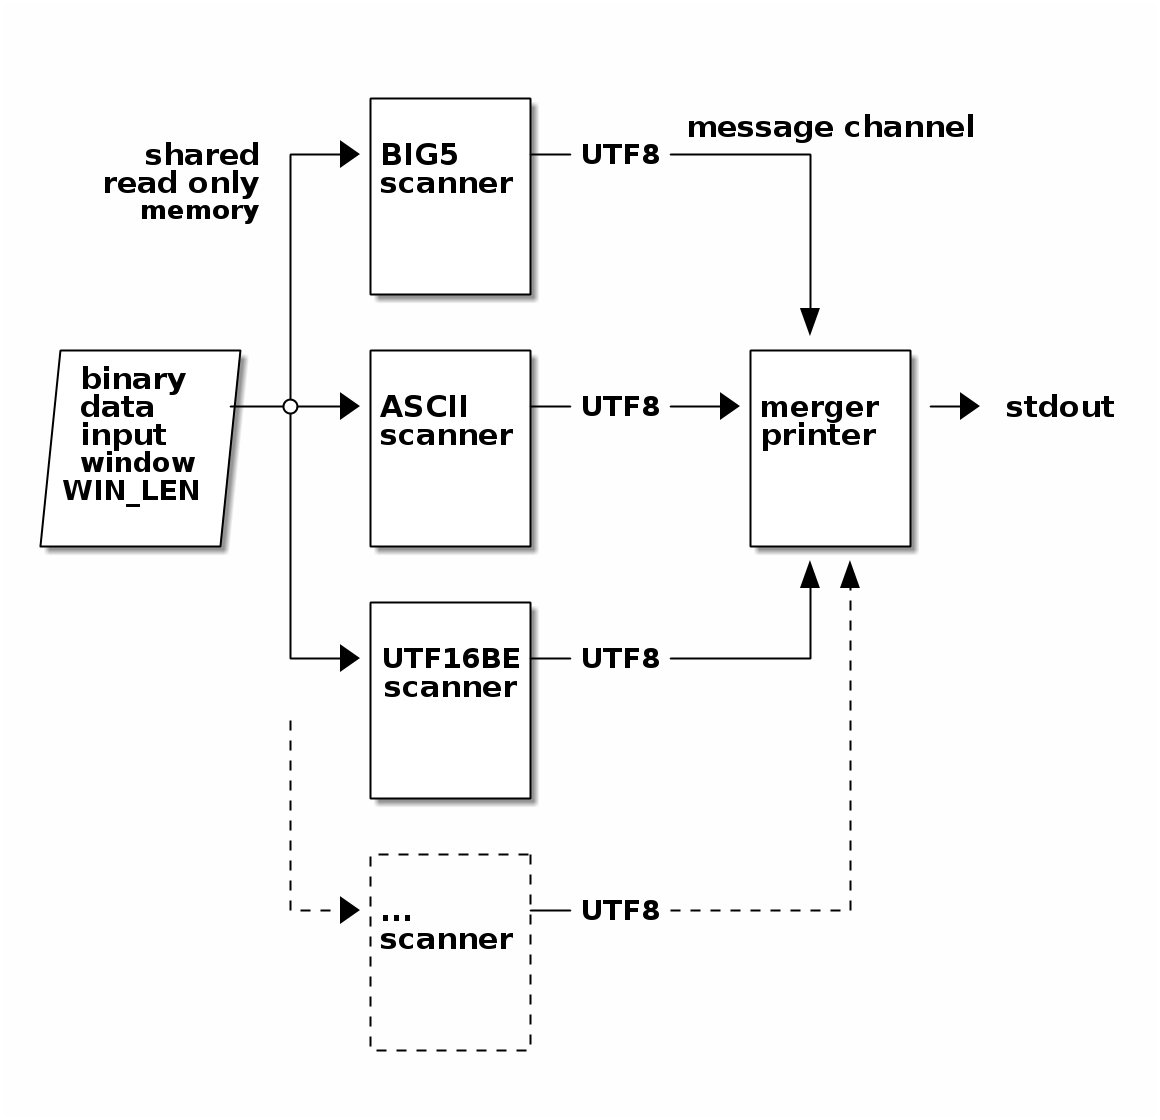
\includegraphics[width=\linewidth]{images/data-processing-and-thread.png.png}
\caption{Data processing and threads}
\label{fig:data-processing-and-threads}
\end{figure}

\subsection{Encoding support}

The initial motivation for developing \emph{Strings­ext} were the
various shortcomings of \emph{GNU-strings} especially when it comes to
handle international character encodings. Does \emph{Strings­ext}
support foreign scripts better? Is it as fast?

To evaluate \emph{Strings­ext}'s capabilities to handle international scripts
with Unicode, we choose the same input text file we used with
\emph{GNU-strings} in the Section, \ref{subsec:test-case-strings} Figure
\ref{fig:test-international-character-encodings}. \emph{Stringsext}'s output
(cf. Figure \ref{fig:stringsext-s-output}) confirms that all international
characters are found correctly.  


\begin{figure}[htbp]
\centering

\includegraphics[width=0.8\linewidth]{images/stringsext-utf-16le-input-cut.png}
    \caption{Strings­ext's output with \texttt{UTF-16LE} encoded input}
    \label{fig:stringsext-s-output}
\end{figure}



\subsection{Deterministic reproducible output}\label{_reproducible_output}

Concurrent computing gives no guarantee in which order partial-output is
available. With regard to \emph{Strings­ext} this means that the order in which
the different scanners report their results, depend on racing conditions which
are not predictable. In order to illustrate this phenomenon, the Figure
\ref{fig:non-reproducible-output} shows the merged output of \emph{Strings­ext}.
It is not surprising that for example at position \texttt{47} and \texttt{c47}
the scanners \emph{ASCII} and \texttt{UTF-8} find the same strings at the same
location since the ASCII-encoding is a subset of the UTF-8 encoding. Whilst at
position \texttt{47} the output of the UTF-8 scanner is first listed, at
position \texttt{c77} the output of the ASCII-scanner is printed first! Even
though the output of \emph{Strings­ext} is always correct, the order in which
the results are listed changes unpredictably!

\begin{figure}[htbp]
\centering
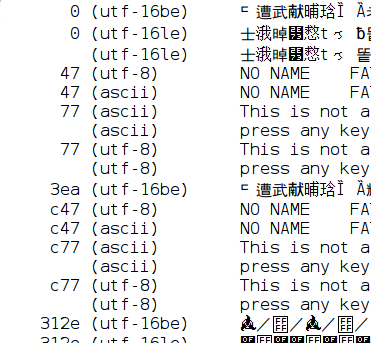
\includegraphics[width=0.6\linewidth]{images/non-reproducible-output.png}
\caption{Output of non deterministic algorithm}
\label{fig:non-reproducible-output}
\end{figure}

The retained solution is to extend the sort criteria by which the
merger thread orders the findings. Now it proceeds as follows: first it sorts
finding by their offsets and then by the encoder name that has reported the
finding. The Figure \ref{fig:reproducible-output} shows the result.  Please note
that for all identical positions the ASCII-scanner result is always listed
first.

\begin{figure}[htbp]
\centering
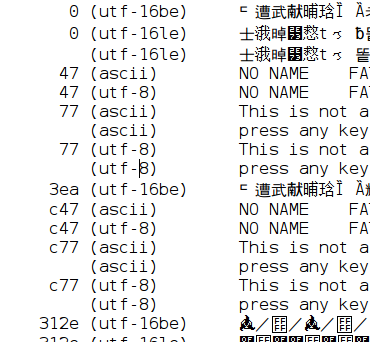
\includegraphics[width=0.6\linewidth]{images/reproducible-output.png}
\caption{Output of deterministic algorithm}
\label{fig:reproducible-output}
\end{figure}

TODO  
TODO  
TODO  
TODO  
TODO  
TODO  
TODO  
TODO  
TODO  
TODO  
TODO  
TODO  
TODO  
TODO  
TODO  
TODO  
TODO  
TODO  
TODO  


\section{Development process evaluation}\label{_development_process_evaluation}

Besides the contribution of the new tool \emph{Strings­ext} to the
forensic community a more general consideration is of scientific
interest: Seeing that Rust is a very young programming language: how
well is the Rust ecosystem suited for forensic tool development?

Forensic tools have to fulfil stringent requirements concerning their quality:
In general, huge amount of data has to be processed which leads to most
demanding requirements in terms code efficiency (cf. Section
\ref{subsec:code-efficiency}).  Furthermore, the data to be analysed is
potentially dangerous: it may contain malicious payload targeting common
vulnerabilities (cf. Section \ref{subsec:security1}).  Finally, in order to
fulfil legal requirements forensic tools must be extensively tested.

The present case study confirms our initial hypothesis that Rust addresses these
requirements: Rust, as system programming language, is designed for code
efficiency. Rust's security guaranties comprise memory safety, the cause for a
common category of vulnerabilities. It's build in unit testing feature supports
\emph{software verification} as defined in the Section
\ref{subsec:tool-validation}.

Guaranteed memory safety is a core property of Rust's borrow checker:
When a Rust source code compiles, the resulting binary \emph{is}
guaranteed to be memory safe. In consequence, such a binary is immune to
memory safety related attacks: e.g. out-of-bounds read, buffer
over-read, heap-based buffer overflow, improper validation of array
index, improper release of memory before removing last, double free, use
after free. As \emph{Strings­ext} and all its used libraries are solely
Rust components, \emph{Strings­ext} is memory safe.

We compared the code efficiency of \emph{GNU-strings} implemented in C
and \emph{Strings­ext} implemented in Rust: When \emph{Strings­ext} is
run in ASCII-only mode, both produce the same output. The field
experiment yielded the expected result, 2.4 times slower but still on
the same scale. However, \emph{Stringsext's} design implies much more
complex computations, hence the result is not surprising.

How about the efficiency of Rust's abstractions and its overall performance? A
good estimation is to compare benchmarks of small and simple programs. Too
complex programs should be avoided for this purpose because variations of the
programmer's skills may bias the result.  According to the ``Computer Language
Benchmark Game'' \cite{fulgham2016} Rust and \emph{C/C++} have similar
benchmark results.

Forensic tools have to operate on many architectures. Here enters Rust's
cross-compiling feature on scene.  As \emph{Rust} uses the LLVM framework as
backend, it is available for most platforms. \texttt{rustc --print target-list}
lists 26 compiler targets.

As described above, Rust's memory safety guarantee is a huge improvement in
terms of security because a whole category of potential vulnerabilities can be
ruled out from the outset. But memory safety does not mean bug freeness! Beside
the security aspects discussed above, the correctness of forensic software is
crucial (cf. Section \ref{subsec:tool-validation}). It is clear that the overall
correctness of a program depend also on the correctness of every library used.
Hence, the question arises whether the Rust ecosystem is mature enough to meet
the ambitious requirements of forensic software. Indeed, compared to C, Rust's
libraries are relatively young. Here again extensive unit testing revealed to be
a helpful diagnostic method: version 0.4.16 of the brand new \texttt{kmerge}
function, part of the \texttt{itertools} library used in \emph{Strings­ext},
reversed under rare conditions the first and second finding. This bug was
actually fixed with pull request \#135 (2. Aug.  2016) some days after its
appearance. Although the bug-fix was already committed in Github, the package
manager did not know about it, because no new version of \texttt{itertools} was
released yet. On the whole, a little change in the package reference list
\texttt{Cargo.toml} solved the problem immediately. Finally, it took another
week for the corrected \texttt{itertools} version to be released. So far this
was the only time we encountered a bug in any of the used libraries. One
conclusion we can draw from this experience, is that young libraries are more
likely to have bugs than established ones. It cannot be emphasised enough that,
diligent unit tests help to find most bugs at early state. Also, those present in
external libraries. However, unit testing do not help against memory safety
related vulnerabilities, which are typical for C and C++ programs and which can
persist in software for decades. It is incumbent on readers to form their own
opinion, We largely prefer accepting the greater likelihood of manageable bugs
related to young Rust libraries, than the uncertainty of hidden memory safety
related vulnerabilities typical for \emph{C} and \emph{C++}.

% Rust code has the reputation that it is easy to read and understand, but
% it is hard to write. We subscribe to this point of view. Rust's biggest
% strength is that unsafe code does not compile, can be also very
% frustrating. Especially when you do not understand the compiler's error
% messages. At some stage it even happened, that we run out of ideas how to
% fix a particular problem. Fortunately, the Rust Internet community is
% very supporting and helpful. In the meantime, also Rust's error messages
% improved with version 1.12 and Rust's documentation is steadily updated
% and enhanced.

Finally, we recognize the benefits of \emph{unit testing} throughout this work.
For this reason we chose for this project the \emph{test driven development}
method where \emph{unit testing} is the key element. Contrary to other methods,
in \emph{test driven development} unit tests and the to be tested code is always
programmed by the same person, which fits well the setting of this project.
However, other methods may be as suitable depending on the organisational
structure of the programmer team.

\section{Conclusion}


The use case ``development of the \emph{Stringsext}-tool'' shows that Rust was a
good choice for the present project, even though batch processing of multi-bytes
character streams revealed to be far more complex than expected.  Additionally,
concurrent programming in Rust posed a formidable hurdle at the beginning.
Fortunately, it did prove to be helpful to contact the Rust community for their
friendly assistance. In addition, for a not so experienced Rust programmer it is
reassuring to know that when a complex piece of code finally compiles, it is
memory safe. The same reasoning applies when a programmer has to refactor
existing code. ``We often had a queasy feeling when we had to work on other
people's C code.'' ``Do we free the memory at the right moment? Is this pointer
still valid?'' Rust's ownership paradigm resolves this uncertainty. When it
compiles, then it is memory safe. Furthermore, Rust is especially suitable for
bigger projects where several programmers contribute to the same code. And this
is particularly true when developing forensic software with its high quality
standards.

It has to be noted though that the Rust ecosystem is still very young
and bugs in new libraries are nothing uncommon. Fortunately, the library
maintainers are very responsive and a bug is usually fixed within days.
Here again unit testing becomes handy. It does not only find bugs in our
own code at early stage, it also helps to identity bugs in external
libraries. Used together with the \emph{test driven development} method,
the test code and the to be tested code can be validated in one go.

\emph{Strings­ext} is currently in production state and can be used in forensic
investigations as a \emph{GNU strings} replacement. It is especially useful
where \emph{GNU-strings} fails: for example it allows finding UTF-16 multi-byte
characters in memory images. 

\bibliographystyle{splncs03}
%\bibliography{references}


\begin{thebibliography}{10}
\providecommand{\url}[1]{\texttt{#1}}
\providecommand{\urlprefix}{URL }

\bibitem{beckett2007}
Beckett, J., Slay, J.: Digital forensics: {{Validation}} and verification in a
  dynamic work environment. pp. 266a--266a. {IEEE} (2007)

\bibitem{berinato2007}
Berinato, S.: The {{Rise}} of {{Anti Forensics}}. (Aug 2007),
  \url{http://www.csoonline.com/article/2122329}

\bibitem{secconsult2017}
Consult, S.: Chainsaw of {{Custody}}: {{Manipulating}} forensic evidence the
  easy way (May 2017),
  \url{http://blog.sec-consult.com/2017/05/chainsaw-of-custody-manipulating.html}

\bibitem{mitrecorporation2016}
Corporation, M.: {{CWE}} - {{Common Weakness Enumeration}}, a
  {{Community}}-{{Developed Dictionary}} of {{Software Weakness Types}} (2016),
  \url{https://cwe.mitre.org/}

\bibitem{craiger2006}
Craiger, P., Swauger, J., Marberry, C., Hendricks, C.: Validation of digital
  forensics tools. Digital crime and forensic science in cyberspace. Hershey,
  PA: Idea Group Inc pp. 91--105 (2006)

\bibitem{cygnussolutions1999}
Cygnus-Solutions: Log message: Sourceware import (Mar 1999),
  \url{https://sourceware.org/ml/binutils-cvs/1999-q2/msg00000.html}

\bibitem{eggendorfer2016}
Eggendorfer, T.: {{IT}} forensics. {{Why}} post-mortem is dead. {{Cyber
  Security Summer School}} 2016: {{Digital Forensics}}, {{Technology}} and
  {{Law}} (Jul 2016)

\bibitem{fulgham2016}
Fulgham, B., Gouy, I.: Computer {{Language Benchmarks Game}}: {{C}}++
  versus~{{Rust}} (Oct 2016), \url{http://benchmarksgame.alioth.debian.org}

\bibitem{getreu2017a}
Getreu, J.: Stringsext, a {{GNU Strings Alternative}} with
  {{Multi}}-{{Byte}}-{{Encoding Support}} (Sep 2017),
  \url{https://github.com/getreu/stringsext}

\bibitem{getreu2017}
Getreu, J.: Forensic-{{Tool Development}} with {{Rust}}. Master's thesis, Tallinn
  University of Technology, Tallinn (Mar 2017),
  \url{http://blog.getreu.net/\_downloads/forensic-tool-development-with-rust.pdf}

\bibitem{harichandran2016}
Harichandran, V.S., Walnycky, D., Baggili, I., Breitinger, F.: {{CuFA}}: {{A}}
  more formal definition for digital forensic artifacts. Digital Investigation
  18,  S125--S137 (2016)

\bibitem{the-rust-project-developers2017}
{The-Rust-Project-Developers}: The {{Rustonomicon}} (2017),
  \url{https://doc.rust-lang.org/nomicon/}

\bibitem{zalewski2014}
Zalewski, M.: {{PSA}}: Don't run 'strings' on untrusted files
  ({{CVE}}-2014-8485) (Oct 2014),
  \url{http://lcamtuf.blogspot.com.ee/2014/10/psa-dont-run-strings-on-untrusted-files.html}

\end{thebibliography}


\end{document}
